% Author: Izaak Neutelings (Februari, 2020)

\documentclass[border=3pt,tikz]{standalone}
\usepackage{amsmath} % for \dfrac
\usepackage{physics,siunitx}
\usepackage{tikz,pgfplots}
\usepackage[outline]{contour} % glow around text
\contourlength{1.0pt}
\usetikzlibrary{angles,quotes} % for pic (angle labels)
\usetikzlibrary{arrows.meta}
\usetikzlibrary{decorations.markings}
\tikzset{>=latex} % for LaTeX arrow head
\usepackage{xcolor}
\colorlet{Rcol}{green!60!black}
\colorlet{Ccol}{orange!90!black}
\colorlet{Lcol}{violet!90}
\colorlet{Icol}{blue!60!black}
\colorlet{myblue}{blue!70!black}
\colorlet{myred}{red!70!black}
\colorlet{Ecol}{orange!90!black}
\tikzstyle{Rline}=[Rcol,thick]
\tikzstyle{gline}=[Rcol,thick]
\tikzstyle{bline}=[myblue,thick]
\tikzstyle{rline}=[myred,thick]
\tikzstyle{width}=[{Latex[length=5,width=3]}-{Latex[length=5,width=3]},thick]
\def\xmax{5.5}
\def\ymax{1.6}
\def\A{1.2}
\def\I{1.1}
\def\om{(395/(0.94*\xmax))}
\def\tick#1#2{\draw[thick] (#1) ++ (#2:0.03*\ymax) --++ (#2-180:0.06*\ymax)}
\newcommand\EMF{\mathcal{E}} %\varepsilon}


\begin{document}



% AC circuit R
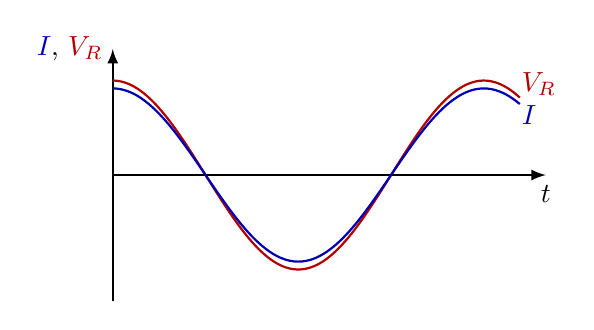
\begin{tikzpicture}
  \coordinate (O) at (0,0);
  \coordinate (X) at (\xmax,0);
  \coordinate (Y) at (0,\ymax);
  
  % AXIS
  \draw[->,thick]
    (0,-\ymax) -- (Y) node[left] {{\color{myblue}$I$}, {\color{myred}$V_R$}};
  \draw[->,thick]
    (O) -- (X) node[below] {$t$};
  
  % PLOT
  \draw[rline,samples=100,smooth,variable=\x,domain=0:0.94*\xmax]
    plot(\x,{\A*cos(\om*\x)}) node[above right=-3] {$V_R$};
  \draw[bline,samples=100,smooth,variable=\x,domain=0:0.94*\xmax]
    plot(\x,{\I*cos(\om*\x)}) node[below right=-3] {$I$};
  	
\end{tikzpicture}



% AC circuit C
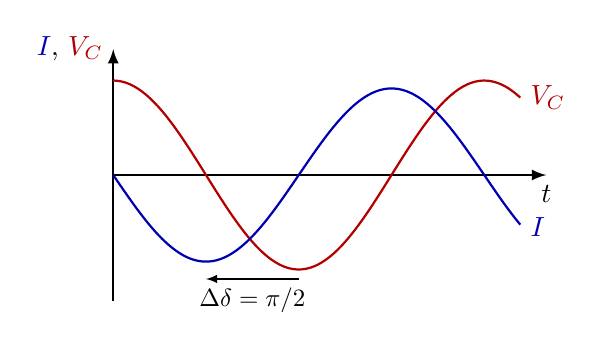
\begin{tikzpicture}
  \coordinate (O) at (0,0);
  \coordinate (X) at (\xmax,0);
  \coordinate (Y) at (0,\ymax);
  
  % AXIS
  \draw[->,thick]
    (0,-\ymax) -- (Y) node[left] {{\color{myblue}$I$}, {\color{myred}$V_C$}};
  \draw[->,thick]
    (O) -- (X) node[below] {$t$};
  
  % PLOT
  \draw[rline,samples=100,smooth,variable=\x,domain=0:0.94*\xmax]
    plot(\x,{\A*cos(\om*\x)}) node[right] {$V_C$};
  \draw[bline,samples=100,smooth,variable=\x,domain=0:0.94*\xmax]
    plot(\x,{\I*cos(\om*\x+90)}) node[below=1,right] {$I$};
  
  % PHASE DIFFERENCE
  \draw[<-]
    ({90/\om},-1.1*\A) --++ ({90/\om},0)
    node[midway,below,scale=0.9] {$\Delta\delta = \pi/2$}; %{$\dfrac{\pi}{2}$}; fill=white,inner sep=1
  	
\end{tikzpicture}


% AC circuit L
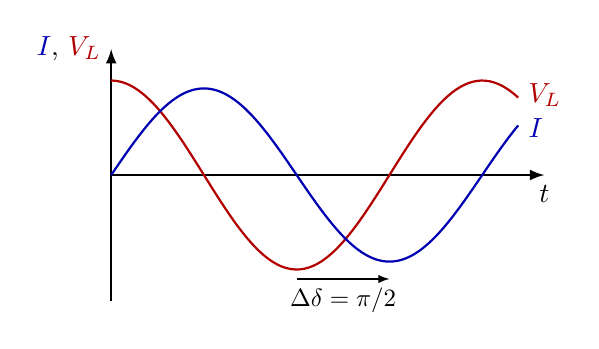
\begin{tikzpicture}
  \coordinate (O) at (0,0);
  \coordinate (X) at (\xmax,0);
  \coordinate (Y) at (0,\ymax);
  
  % AXIS
  \draw[->,thick]
    (0,-\ymax) -- (Y) node[left] {{\color{myblue}$I$}, {\color{myred}$V_L$}};
  \draw[->,thick]
    (O) -- (X) node[below] {$t$};
  
  % PLOT
  \draw[rline,samples=100,smooth,variable=\x,domain=0:0.94*\xmax]
    plot(\x,{\A*cos(\om*\x)}) node[above=1,right] {$V_L$};
  \draw[bline,samples=100,smooth,variable=\x,domain=0:0.94*\xmax]
    plot(\x,{\I*cos(\om*\x-90)}) node[below=1,right] {$I$};
  
  % PHASE DIFFERENCE
  \draw[->]
    ({180/\om},-1.1*\A) --++ ({90/\om},0)
    node[midway,below,scale=0.9] {$\Delta\delta = \pi/2$};
  
\end{tikzpicture}


% AC circuit LCR in series
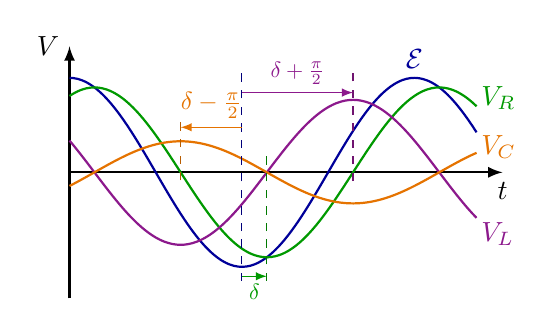
\begin{tikzpicture}
  \def\om{(425/(0.94*\xmax))}
  \def\del{26}
  \def\VR{\A*cos(\del)}
  \def\f{0.3}
  \def\X{\A*sin(\del)/(1-2*\f)}
  \coordinate (O) at (0,0);
  \coordinate (X) at (\xmax,0);
  \coordinate (Y) at (0,\ymax);
  
  % AXIS
  \draw[->,thick]
    (0,-\ymax) -- (Y) node[left] {$V$}; %{{\color{myblue}$I$}, {\color{myred}$V_L$}};
  \draw[->,thick]
    (O) -- (X) node[below] {$t$};
  
  % PLOT
  \draw[Icol,thick,samples=100,smooth,variable=\x,domain=0:0.94*\xmax]
    plot(\x,{\A*cos(\om*\x)}); % node[right=-1] {$\EMF$};
  \node[Icol,above] at ({360/\om},\A) {$\EMF$};
  \draw[Rcol,thick,samples=100,smooth,variable=\x,domain=0:0.94*\xmax]
    plot(\x,{\VR*cos(\om*\x-\del)}) node[below=3,above right=-2] {$V_R$}; % = R\EMF/Z %\frac{R}{Z}
  \draw[Lcol,thick,samples=100,smooth,variable=\x,domain=0:0.94*\xmax]
    plot(\x,{(1-\f)*\X*cos(\om*\x-\del+90)}) node[below right=-2] {$V_L$};
  \draw[Ccol,thick,samples=100,smooth,variable=\x,domain=0:0.94*\xmax]
    plot(\x,{\f*\X*cos(\om*\x-\del-90)}) node[above=2,right=-2] {$V_C$};
  
  % PHASE DIFFERENCE
  \draw[Icol!80!black,dashed] ({180/\om},-1.15*\A) -- ({180/\om},1.05*\A);
  \draw[Rcol!80!black,dashed] ({(180+\del)/\om},-1.15*\A) -- ({(180+\del)/\om},{0.2*\VR});
  \draw[Lcol!80!black,dashed] ({(270+\del)/\om},{-0.12*(1-\f)*\X}) -- ({(270+\del)/\om},{1.46*(1-\f)*\X});
  \draw[Ccol!80!black,dashed] ({( 90+\del)/\om},{-0.26*\f*\X}) -- ({(90+\del)/\om},{1.64*\f*\X});
  \draw[->,Rcol]
    ({180/\om},-1.1*\A) --++ ({\del/\om},0)
    node[midway,below,scale=0.8] {$\delta$}; %\Delta\delta = 
  \draw[->,Lcol]
    ({180/\om},{1.1*(1-\f)*\X}) --++ ({(\del+90)/\om},0)
    node[midway,above,scale=0.8] {$\delta + \frac{\pi}{2}$}; %\Delta\delta = 
  \draw[->,Ccol]
    ({180/\om},{1.45*\f*\X}) --++ ({(\del-90)/\om},0)
    node[midway,above,scale=0.9] {$\delta - \frac{\pi}{2}$};
  
\end{tikzpicture}


% RESONATE
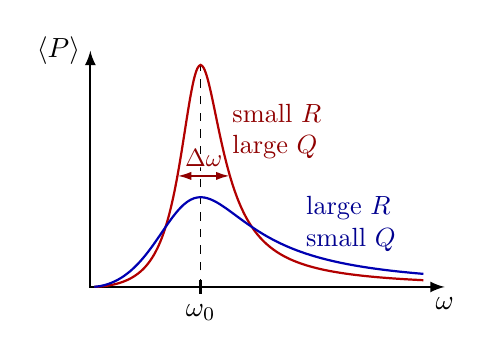
\begin{tikzpicture}
  \def\xmax{4.5}
  \def\ymax{3}
  \def\c{1.4}
  \def\a{0.38*\ymax}
  \def\A{0.94*\ymax}
  \def\q{0.9}
  \def\Q{2.1}
  \def\t{360/(0.94*\xmax)}
  \coordinate (O) at (0,0);
  \coordinate (X) at (\xmax,0);
  \coordinate (Y) at (0,\ymax);
  \coordinate (C) at (\c,0);
  
  % AXIS
  \draw[<->,thick]
    (Y) node[left] {$\langle{P}\rangle$} -- (0,0) -- (X) node[below] {$\omega$};
  \draw[dashed,thin] (C) --++ (0,\A);
  \tick{C}{90} node[below] {$\omega_0$};
  
  % PLOT
  \draw[rline,samples=100,smooth,variable=\x,domain=0.05:0.94*\xmax]
    plot(\x,{\A/( (\Q*(\x^2-\c^2)/(\x*\c))^2 + 1 )});
  \draw[bline,samples=100,smooth,variable=\x,domain=0.05:0.94*\xmax]
    plot(\x,{\a/( (\q*(\x^2-\c^2)/(\x*\c))^2 + 1 )});
  \node[myred!80!black,align=left,right,scale=0.95] at (\c+0.6/\Q,0.7*\A) {small $R$\\large $Q$};
  \node[myblue!80!black,align=left,right,scale=0.95] at (\c+1.1/\q,0.7*\a) {large $R$\\small $Q$};
  
  % WIDTH
  %\draw[<->,thick] ({\c/(2*\Q)*(-1+sqrt(1+4*\Q^2))},\A/2) -- ({\c/(2*\Q)*(1+sqrt(1+4*\Q^2))},\A/2);
  %\draw[width,myblue!80!black]
  %  ({\c/(2*\q)*(-1+sqrt(1+4*\q^2))},\a/2) --++ (\c/\q,0) node[midway,above] {$\Delta \omega$};
  \draw[width,myred!80!black]
    ({\c/(2*\Q)*(-1+sqrt(1+4*\Q^2))},\A/2) --++ (\c/\Q,0)
    node[midway,above,scale=0.9] {\contour{white}{$\Delta \omega$}};
  
\end{tikzpicture}


\end{document}
